\section{Algorithms for Computing Minimal Unsatisfiable Subset}
\label{sec:algorithms for computing minimal unsatisfiable subset}
The approach of computing all MUSes of $\varphi$ is to first find all MCSes($\varphi$) and then to compute all irreducible hitting sets of MCSes($\varphi$), which are all MUSes($\varphi$). So, there are two phases to generate all MUSes of a unsatisfiable CNF formula. The first phase is to compute MCSes by using an algorithm and the second phase is to compute MUSes from the MCSes by using a recursive algorithm which authors have developed to compute irreducible hitting sets.\newline
In the first phase, authors use a SAT solver (produces an satisfying assignment, if exists) to work with the input given and generate hitting sets of MUSes (MCSes) without revealing the underlying MUSes. For the second phase, they get all the information with MCSes and use an recursive algorithm to compute minimal and irreducible hitting sets of MCSes (MUSes). 
\begin{Algorithm}
	\caption{Algorithm for finding all MCSes of a formula $\varphi$}
	\label{alg:findmcses}
	\begin{algorithm}{\text{MCSes}}{\text{$\varphi$}}
		\varphi^{\prime} \= AddYVars(\varphi) \\
		MCSes\=\emptyset \\
		k\=1 \\
		\begin{WHILE}{\text{SAT($\varphi$)}}
			\varphi^{\prime}_{k} \= \varphi^{\prime} \wedge AtMost(\{\neg w_{1}, \neg w_{2},\ldots, \neg w_{n}\},k) \\
			\begin{WHILE}{newMCS \= IncrementalSAT(\varphi^{\prime}_{k})}
				MCSes \= MCSes \cup {newMCS} \\
				\varphi^{\prime}_{k} \= \varphi^{\prime}_{k} \wedge BlockingClause(newMCS) \\
				\varphi^{\prime} \= \varphi^{\prime} \wedge BlockingClause(newMCS) \\
			\end{WHILE} \\
			k\=k+1 \\
		\end{WHILE} \\
		\RETURN MCSes
	\end{algorithm}
\end{Algorithm}
\subsection{Computing MCSes}
In Algorithm $1$, there is a method named $\textbf{MCSes}$ which takes a CNF formula $\varphi$ as input. The goal of this is to find minimal set of clauses whose removal makes $\varphi$ satisfiable. In Line $1$, $\varphi$ is augmented with clause-selector variables by creating $\varphi^{\prime}$. The augmentation increases the number of variables. Also the search space grows for finding a satisfying assignment. Initially, the variable, $\textbf{\textit{MCSes}}$ is empty and  at the end we will get all MCSes in this variable. There is a counter variable, $K$ which is initialized by $1$.\newline
Each iteration of the outer while loop (Lines $4$-$12$) finds an MCS of size $K$, which is incremented by $1$ after each iteration. In Line $5$, a clause is added of the form $AtMost(\{\neg w_{1},\neg w_{2},\ldots,\neg w_{n}\},k)$ to $\varphi^{\prime}$ and a new formula, $\varphi^{\prime}_{\text k}$ is created. $K$ number of variables, $w_{i}$ are assigned to $false$ so that $K$ number of clauses could be disabled. The set of variables, $w_{i}$ are assigned to $false$ by indicating the clauses as an MCS.\newline
The inner while loop (Lines $6$-$10$) searches all the satisfiable assignments of $\varphi^{\prime}_{\text k}$ and also finds all MCSes of size $k$. In Line $6$, \textbf{IncrementalSAT} method is called which uses MiniSAT (a modern open-source SAT solver which has incremental solving ability) for finding a solution of $\varphi^{\prime}_{\text k}$. In this method the solving function is invoked multiple times, but each time with a different set of assumption literals and then the solver checks the satisfiability of all the clauses provided with the current assumptions only \cite{nadel}. Each satisfying assignment produces an MCS stored in a variable $\textbf{\textit{newMCS}}$ which contains the clauses having $w_{\text i}$ assigned $false$. Each $\textbf{\textit{newMCS}}$ is recorded in $\textbf{\textit{MCSes}}$ (Line $7$). In Line $8$ and $9$, a blocking clause is added to $\varphi^{\prime}_{k}$ and $\varphi^{\prime}$, respectively to block that solution. Blocking clause is a clause containing the clause-selector variables which consist in the clauses of that MCS. It means at least one of the clauses in the MCS will be enabled for future solution. For example, an MCS has the clauses $C_{2}$ and $C_{3}$ which means $w_{2}$ and $w_{3}$ are assigned false in satisfying assignment. Then the blocking clause will be $(w_{2}\vee w_{3})$. $True$ is assigned to at least one $w_{i}$ excluding the MCS and any of its supersets from any future solution.\newline
All founded MCSes are irreducible as the MCSes were found in increasing size and all supersets are excluded form the future solutions. After evaluating all the solutions with bound $K$ enforces to find solutions with bound $K+1$. Also, $K+1$ disabled clause to be irreducible as potential subsets would have found and blocked.\newline
The outer while loop checks if $\varphi^{\prime}$ is still satisfiable without any bound on $w_{\text i}$. Note that, $\varphi^{\prime}$ is augmented with all  generated blocking clauses. Finding no satisfying assignments indicates that we have found all MCSes and there is no other way to remove clauses for satisfying formula. Finally, the algorithm terminates and returns all MCSes to caller.
\begin{example}
Let us consider, our example formula $\varphi=(x)\wedge(\neg x)\wedge(\neg x\vee y)\wedge(\neg x \vee \neg y)$. So, $\varphi^{\prime}=(\neg w_{1}\vee x)\wedge(\neg w_{2}\vee \neg x)\wedge(\neg w_{3}\vee \neg x\vee y)\wedge(\neg w_{4}\vee \neg x \vee \neg y)$. Initially, $MCSes=\emptyset$ and $k=1$.\newline
In the first iteration, it will add an AtMost bound with $K=1$ by creating $\varphi^{\prime}_{1}=\varphi^{\prime} \wedge AtMost(\{l_{1},l_{2},l_{3},l_{4}\},1)$. At first $false$ is assigned to $w_{1}$ and the incremental solver find a solution for $\varphi^{\prime}_{\text k}$. Now, we get the followings:
$$MCSes=\{C_{1}\}$$
$$\varphi^{\prime}_{1}=\varphi^{\prime}_{1} \wedge w_{1}$$
$$\varphi^{\prime}=\varphi^{\prime} \wedge w_{1}$$
After adding the blocking clause, $(w_{1})$ the incremental solver will be unable to find any further solution with $K=1$. There is no other way to remove one clause to satisfy $\varphi$. It means no other single clause covers all of its MUSes. The inner while loop is exited.\newline
As $\varphi^{\prime}$ is still satisfiable, the bound is incremented to 2 and the search for soluitons of $\varphi^{\prime}_{2}=\varphi^{\prime} \wedge AtMost(\{l_{1},l_{2},l_{3},l_{4}\},2)$ is continued.For $K=2$, we get the followings, respectively:
\begin{itemize}
	\item $w_{2}=false$ and $w_{3}=false,$
	$$MCSes=\{\{C_{1}\}, \{C_{2}, C_{3}\}\}$$
	$$\varphi^{\prime}_{2}=\varphi^{\prime}_{2} \wedge (w_{2}\vee w_{3})$$
	$$\varphi^{\prime}=\varphi^{\prime} \wedge (w_{2}\vee w_{3})$$
	\item $w_{2}=false$ and $w_{4}=false,$
	$$MCSes=\{\{C_{1}\}, \{C_{2}, C_{3}\}, \{C_{2}, C_{4}\}\}$$
	$$\varphi^{\prime}_{2}=\varphi^{\prime}_{2} \wedge (w_{2}\vee w_{4})$$
	$$\varphi^{\prime}=\varphi^{\prime} \wedge (w_{2}\vee w_{4})$$
\end{itemize}
We will not get any other MCSes for $K=2$. Also, the outer while loop will exit as $\varphi^{\prime}$ with all the added blocking clauses is no longer satisfiable. So, final MCSes are, $\{C_{1}\}, \{C_{2}, C_{3}\}$ and $\{C_{2}, C_{4}\}$.
\end{example}
\begin{table}[]
	\centering
	\caption{Running MCSes($\varphi$) on our example formula $\varphi$}
	\label{running-mCSes}
	\begin{tabular}{|c|c|c|c|c|}
		\hline
		\begin{tabular}[c]{@{}l@{}}Step\\ No.\end{tabular} &                & $k$                  & $\varphi^{\prime}$ & MCSes \\ \hline
		1                                                  & Initialization & \multirow{2}{*}{1} & $(x)\wedge (\neq x)\wedge (\neq x \vee y)\wedge (\neq x \vee \neq y) $ & $\emptyset$     \\ \cline{1-2} \cline{4-5} 
		2                                                  & Run1           &                    & $\varphi^{\prime}(step1)\wedge w_{1}$ & $\{C_{1}\}$     \\ \hline
		3                                                  & Run2           & \multirow{2}{*}{2} & $\varphi^{\prime}(step2)\wedge (w_{2}\vee w_{3})$ & $\{C_{2}, C_{3}\}$     \\ \cline{1-2} \cline{4-5} 
		4                                                  & Run3           &                    & $\varphi^{\prime}(step3)\wedge (w_{2}\vee w_{4})$ & $\{C_{2}, C_{4}\}$     \\ \hline
	\end{tabular}
\end{table}
\subsection{Compuitng MUSes}
Once the entire collection of MCSes has been computed, the second phase produces all MUSes of the given instances and this phase is independent of first phase as it does not depend on the semantics of the input of Algorithm $1$. The second phase can be applied to any minimal hitting set. Authors presented a recursive algorithm which takes two inputs, one is set of MCSes and another the MUS currently being constructed in each branch of the recursion. The outputs are all MUSes.\newline
\begin{Algorithm}
\caption{Algorithm for computing the complete set of MUSes from a set of MCSes}
\label{alg:allmuses}
	\begin{algorithm}{\text{AllMUSes}}{\text{MCSes, currentMUS}}
		\begin{IF}{\text{MCSes = $\emptyset$}}
			\text{print(currentMUS)} \\
			\RETURN
		\end{IF}
		\begin{FOR}{\textbf{each} \text{selClause $\varepsilon$ RemainingClauses(MCSes)}} \\
			newMUS \= currentMUS \cup selClause \\
			\begin{FOR}{\textbf{each} \text{selMCS $\varepsilon$ MCSes such that selClause $\varepsilon$ selMCS}} \\
				newMCSes \= MCSes \\
				PropagateChoise(newMCSes, selClause, selMCS) \\
				AllMUSes(newMCSes, newMUS) \\
			\end{FOR}
		\end{FOR}
		\RETURN
	\end{algorithm}
\end{Algorithm}
Algorithm $2$ is the recursive algorithm where the inputs are $\textbf{\textit{MCSes}}$ and $\textbf{\textit{currentMUS}}$. The goal of this is to find a irreducible set of clauses that hits each set of $\textbf{\textit{MCSes}}$. The terminating condition of the recursion is on Line $1$ that is if $\textbf{\textit{MCSes}}$ is empty. If it is,prints the MUS generated in current recursion branch and returns to look for other MUSes in another branches on Line $2$ and in Line $3$,respectively. Lines $5-12$ is iterated through all possible choices of clause selected on Line $5$ and recorded in a variable, $\textbf{\textit{selClause}}$. In Line $6$, $\textbf{\textit{selClause}}$ is stored in a growing MUS, $\textbf{\textit{newMUS}}$. For all possible choices of MCSes (selected on line $7$) recorded in $\textbf{\textit{selMCS}}$ such that $\textbf{\textit{selClause}}$ consists in $\textbf{\textit{selMCS}}$, iteration occurs from Lines $7-11$. Then, $\textbf{\textit{MCSes}}$ is recorded in a variable, $\textbf{\textit{newMCSes}}$.\newline
For every $\textbf{\textit{selMCS}}$ a method, $\textbf{PropagateChoice}$ (Algorithm $3$) is called with $\textbf{\textit{newMCSes}}$, $\textbf{\textit{selClause}}$ and $\textbf{\textit{selMCS}}$.
\begin{figure}[htb] % where to insert the figure: h=here, t=top, b=bottom,
	% the order htb shows which position is preffered
	\begin{center}
		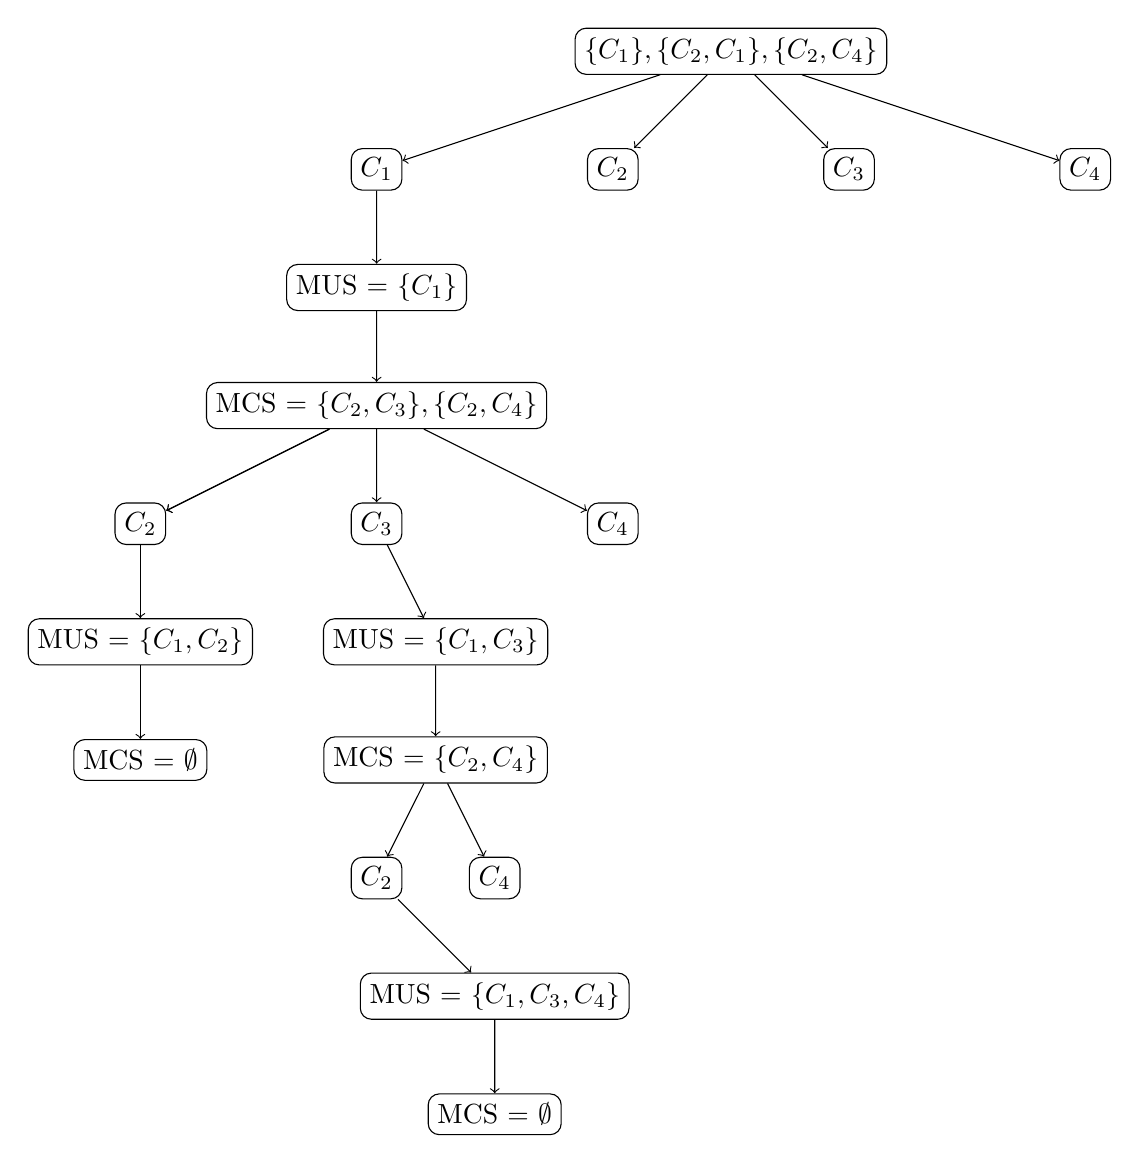
\begin{tikzpicture}[scale=1.5, 
				    state/.style={draw, rounded corners, fill=none,
				    			  text centered, text=black}]
	\node[state] (u1) at (5, 11) {$\{C_{1}\}, \{C_{2},C_{1}\}, \{C_{2},C_{4}\}$};
	\node[state] (u2) at (2, 10) {$C_{1}$};
	\node[state] (u3) at (4, 10) {$C_{2}$};
	\node[state] (u4) at (6, 10) {$C_{3}$};
	\node[state] (u5) at (8, 10) {$C_{4}$};
	\node[state] (u6) at (2, 9) {MUS = $\{C_{1}\}$};
	\node[state] (u7) at (2, 8) {MCS = $\{C_{2}, C_{3}\}, \{C_{2}, C_{4}\}$};
	\node[state] (u8) at (0, 7) {$C_{2}$};
	\node[state] (u9) at (2, 7) {$C_{3}$};
	\node[state] (u10) at (4, 7) {$C_{4}$};
	\node[state] (u11) at (0, 6) {MUS = $\{C_{1}, C_{2}\}$};
	\node[state] (u12) at (0, 5) {MCS = $\emptyset$};
	\node[state] (u13) at (2.5, 6) {MUS = $\{C_{1}, C_{3}\}$};
	\node[state] (u14) at (2.5, 5) {MCS = $\{C_{2}, C_{4}\}$};
	\node[state] (u15) at (2, 4) {$C_{2}$};
	\node[state] (u16) at (3, 4) {$C_{4}$};
	\node[state] (u17) at (3, 3) {MUS = $\{C_{1}, C_{3}, C_{4}\}$};
	\node[state] (u18) at (3, 2) {MCS = $\emptyset$};
	
	\path[->] 	(u1)  edge   (u2);
	\path[->] 	(u1)  edge   (u3);
	\path[->] 	(u1)  edge   (u4);
	\path[->] 	(u1)  edge   (u5);
	\path[->] 	(u2)  edge   (u6);
	\path[->] 	(u6)  edge   (u7);
	\path[->] 	(u7)  edge   (u8);
	\path[->] 	(u7)  edge   (u8);
	\path[->] 	(u7)  edge   (u9);
	\path[->] 	(u7)  edge   (u10);
	\path[->] 	(u8)  edge   (u11);
	\path[->] 	(u11)  edge   (u12);
	\path[->] 	(u9)  edge   (u13);
	\path[->] 	(u13)  edge   (u14);
	\path[->] 	(u14)  edge   (u15);
	\path[->] 	(u14)  edge   (u16);
	\path[->] 	(u15)  edge   (u17);
	\path[->] 	(u17)  edge   (u18);
	
\end{tikzpicture}

	\end{center}
	\caption{Illustration of all MUSes}
	\label{fig:graphallmuses}
\end{figure}
\begin{Algorithm}
	\caption{Algorithm for altering MCSes to make the choice of thisClause irredundant as the only element hitting thisMCS}
	\label{alg:propagatechoise}
	\begin{algorithm}{\text{PropagateChoice}}{\text{MCSes, thisClause, thisMCS}}
		\begin{FOR}{\textbf{each} \text{clause $\varepsilon$ thisMCS}}
			\begin{FOR}{\textbf{each} \text{testMCS $\varepsilon$ MCSes}}
				\begin{IF}{\text{clause $\varepsilon$ testMCS}}
					testMCS \= testMCS - \{clause\} \\
				\end{IF}
			\end{FOR}
		\end{FOR}
		\begin{FOR}{\textbf{each} \text{testMCS $\varepsilon$ MCSes}}
			\begin{IF}{\text{thisClause $\varepsilon$ testMCS}}
				testMCS \= testMCS - \{clause\} \\
				MCSes \= MCSes - \{testMCS\} \\
			\end{IF}
		\end{FOR}
		MaintainNoSupersets(MCSes)
	\end{algorithm}
\end{Algorithm}
Algorithm $3$ has the goal to alter a copy of the current MCSes $(\textbf{\textit{newMCSes}})$. It alters by removing an MCS from $\textbf{\textit{MCSes}}$ hitted by $\textbf{\textit{thisClause}}$. In the last line, $\textbf{MaintainNoSupersets}$ is invoked which removes any MCS from $\textbf{\textit{MCSes}}$ which is a superset of others. This is needed as we are dealing with the minimal set of MCSes and no MCS cannot be a superset of others. For example, let we have $MCSes=\{\{C_{2}\}\{C_{1}, C_{3}\}\{C_{2},C_{4}\}\}$. Here, $\{C_{2},C_{4}\}$ is a superset of $\{C_{2}\}$. If we pass this MCSes through $\textbf{MaintainNoSupersets}$, $\{C_{2},C_{4}\}$ will be removed.\newline
The recursion of Algorithm $2$ continues by calling $\textbf{AllMUSes}$ with $\textbf{\textit{newMCSes}}$ and $\textbf{\textit{newMUS}}$.
\begin{example}
Let us consider, our example formula $\varphi$. We already have found $MCSes(\varphi)=\{\{C_{1}\}, \{C_{2}, C_{3}\}, \{C_{2}, C_{4}\}\}$. Let, $C_{1}$ is chosen as $\textbf{\textit{selClause}}$ in the first iteration. So, $C_{1}$ is added in the growing MUS. Now, for each set of MCSes another iteration will occur which calls $\textbf{PropagateChoice}$ method by creating a modified copy of current MCSes and makes a recursive call to itself. Modified MCSes contain $\{C_{2}, C_{3}\}\{C_{2},C_{4}\}$. The recursive call continues until empty MCSes is not found. Empty MCSes is found by producing a MUS, $\{C_{2}, C_{3}\}$. Now, it will look for other MUSes in other branches. For our example the whole procedure to generate all MUSes is illustrated in the Figure 2. Finally, we get all MUSes, $\{C_{1}, C_{2}\}$ and $\{C_{1},C_{3}, C_{4}\}$.
\end{example}